\documentclass[tikz,border=5pt]{standalone}
\usepackage[UTF8]{ctex}
\usepackage{amsmath}
\usetikzlibrary{arrows.meta,calc,decorations.pathmorphing,patterns}
\definecolor{blue}{RGB}{45,98,142}
\definecolor{green}{RGB}{60,117,87}
\definecolor{red}{RGB}{175,67,51}
\tikzset{rubber/.style={thick,decorate,decoration={zigzag,amplitude=2pt,segment length=7pt}},force/.style={red,thick,-{Stealth}}}
\begin{document}
\begin{tikzpicture}
\draw[thick](0,-1.15)--(0,1.5);
\draw[rubber](0,.925)--(2.1,.925);\draw[rubber](0,.275)--(2.1,.275);
\draw[thick](2.1,.275)--(2.1,.925);\draw[blue,thick](2.1,.6)--(4,.6);
\draw[rubber](0,-.6)--(2.3,-.6);\draw[blue,thick](2.3,-.6)--(4,-.6);
\draw[gray,thick](4,0)circle(.6);\draw[blue,thick](4,.6)arc(90:-90:.6);
\fill(4,0)circle(2pt);\draw[force](4,0)--(5.5,0)node[right]{$F$};
\node at(1,1.25){$k$};\node at(1,-.05){$k$};\node at(1,-.95){$k$};
\draw[gray,<->](3.5,-1.15)--node[below]{$X$}(4,-1.15);
\begin{scope}[xshift=7.2cm]
\draw[fill=blue!6](0,-.15)--(3,-.55)--(3,.55)--(0,.15)--cycle;
\draw[gray](0,.15)--(.18,.3)--(3.18,.7)--(3,.55);
\draw[gray](3.18,.7)--(3.18,-.4)--(3,-.55);
\node at(-.4,0){$S_1$};\node at(3.55,0){$S_2$};
\draw[gray,<->](0,-.95)--node[below]{$l_0$}(3,-.95);
\node[align=center]at(1.5,1.35){截面积沿长度线性变化\\图示为恒厚度变宽条带};
\end{scope}
\node at(4.8,-1.85){轮缘连接相切；并联组与第三根由同一轻绳相连};
\end{tikzpicture}
\begin{tikzpicture}
\draw[thick](0,-1.2)--(0,1.2);
\draw[blue,thick](0,.6)--(3,.6)arc(90:-90:.6)--(0,-.6);
\draw[gray](3,0)circle(.6);\fill(3,0)circle(2pt);
\draw[force](3,0)--(4.5,0)node[right]{$F$};
\draw[force](2.8,.6)--(1.65,.6)node[above]{$T$};
\draw[force](2.8,-.6)--(1.65,-.6)node[below]{$T$};
\draw[blue,-{Stealth}](3,-1.05)--(3.85,-1.05)node[right]{$X$};
\node[align=center]at(2.2,-2.0){$F=2T$\\$\delta_{\parallel}+\delta_3=2X$};
\node at(1.1,1.25){上股接并联段};\node at(1.1,-1.2){下股接第三根};
\end{tikzpicture}
\begin{tikzpicture}
\foreach \y in{-.45,0,.45}{\draw[rubber](0,\y)--(2,\y);}
\draw[thick](0,-.6)--(0,.6);\draw[thick](2,-.6)--(2,.6);\draw[thick](2,0)--(2.5,0);
\foreach \y in{-.3,.3}{\draw[rubber](2.5,\y)--(4.5,\y);}
\draw[thick](2.5,-.45)--(2.5,.45);\draw[thick](4.5,-.45)--(4.5,.45);
\draw[thick](4.5,0)--(5,0);\draw[rubber](5,0)--(7,0);
\draw[force](0,0)--(-.8,0)node[left]{$F$};\draw[force](7,0)--(7.8,0)node[right]{$F$};
\node at(1,1){$A:\ 9k$};\node at(3.5,1){$B:\ 6k$};\node at(6,1){$C:\ 3k$};
\node[align=center]at(3.5,-1.1){每根原长 $l_0/3$，单根刚度 $3k$\\三段总拉力均为 $F$，总伸长逐段相加};
\end{tikzpicture}
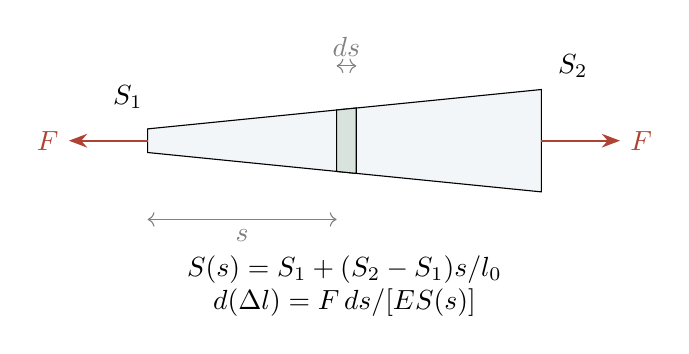
\begin{tikzpicture}
\draw[fill=blue!6](0,-.15)--(5,-.65)--(5,.65)--(0,.15)--cycle;
\draw[fill=green!20](2.4,-.39)--(2.65,-.415)--(2.65,.415)--(2.4,.39)--cycle;
\draw[force](0,0)--(-1,0)node[left]{$F$};\draw[force](5,0)--(6,0)node[right]{$F$};
\node at(-.25,.55){$S_1$};\node at(5.4,.95){$S_2$};
\draw[gray,<->](0,-1)--node[below]{$s$}(2.4,-1);
\draw[gray,<->](2.4,.95)--node[above]{$ds$}(2.65,.95);
\node[align=center]at(2.5,-1.85){$S(s)=S_1+(S_2-S_1)s/l_0$\\$d(\Delta l)=F\,ds/[ES(s)]$};
\end{tikzpicture}
\begin{tikzpicture}
\draw[thick](-1,.15)--(1,.15);\draw[thick](0,.15)--(0,0);
\draw[fill=blue!6](-.25,0)--(-.7,-4)--(.7,-4)--(.25,0)--cycle;
\draw[fill=green!18](-.43,-1.6)--(-.7,-4)--(.7,-4)--(.43,-1.6)--cycle;
\draw[thick](-.43,-1.6)--(.43,-1.6);
\draw[force](0,-1.6)--(0,-.75)node[right]{$N(s)$};
\draw[force](0,-2.8)--(0,-3.7);
\node[red,right]at(1.7,-3.3){$W_{\rm below}(s)$};
\draw[blue,-{Stealth}](1.1,0)--(1.1,-4.3)node[right]{$s$};
\node at(-.7,-.25){$S_1$};\node at(-1.05,-3.9){$S_2$};
\node[right]at(1.1,-1.6){截面 $s$};
\node[align=center]at(.2,-5.15){$W_{\rm below}(s)=\rho g\int_s^{l_0}S(\xi)d\xi$\\自由端 $N(l_0)=0$；截面拉力等于阴影段重量};
\end{tikzpicture}
\end{document}
